\externaldocument{../appendix/chapter_app}
\startchapter{Communication Modeling}
\label{chapter:mod}
In this chapter, I depict the model of the communication of two running programs from the trace analysis point of view. The modeling is based on the investigation of some common used communication methods. But the detail of the communication methods will be discussed later in the algorithm and implementation chapters. This chapter only present the abstract communication model regarding to the two communication categories: reliable and unreliable communications. 

\section{Communication Methods Categorization}
In general,  in the terms of their reliability of data transmission, there are two types of communication: reliable and unreliable. A reliable communication guarantees the data being sent by one endpoint through the channel is always received losslessly and in the same order in the other endpoint. On contrast, an unreliable communication does not guarantee the data being sent always arrive the receiver. Moreover, the data packets can arrive to the receiver in any order. However, the bright side of unreliable communication is that the packets being sent are always arrived as the origin packet, no data re-segmentation would happen. An endpoint is an instance in a program at which a stream of data is sent or a stream of data is received or both (e.g. socket handle of TCP or a file handle of the named pipe). A channel is a conduit connected two endpoints through  which data can be sent and received. Table\ref{methodsInCategories} gives examples of communication methods fall in these two categories.
\begin{table}[H]
\centering
\caption{Communication Method Examples in Two Categories}
\label{methodsInCategories}
\begin{tabular}{|l|l|}
 \hline
\textbf{Reliable Communication}& \textbf{Unreliable Communication}\\
 \hline
Named Pipes & Message Queue   \\
TCP &  UDP \\
 \hline
\end{tabular}
\end{table}


\section{Communication Model}\label{definition}
The communication of two programs is defined in this section. The communication in this work is data transfer activities between two running programs through a specific channel. Some collaborative activities between the programs such as remote procedure call is out of the scope of this research. Communication among multiple programs (more than two) is not discussed in this work. The channel can be reopened again to start new communications after being closed. However, the reopened channel is considered as a new communication. The way that I define the communication is leading to the communication analysis in the dual-trace. So the definition is not about how the communication works but what it looks like. There are many communication methods in the real world and they are compatible to this communication definition. 

\subsection{Communication Definition}
In the context of a dual\_trace, a communication is a sequence of data transmitted of two endpoints through a communication channel. The endpoints connect to each other using the identifier of this channel. We therefore defined a communication $c$ as a triplet:

$c =<ch, e_0, e_1>$

where $e_0$ and $e_1$ are endpoints while $ch$ is the communication channel (e.g. a named piped located at /tmp/pipe).

From the point of view of traces, the endpoints $e_0$ and $e_1$ are defined in terms of three properties: the handle created within a process for the endpoint for subsequent operations(e.g. data send and receive), the data stream received and the data stream sent. Therefore, I define an endpoint $e$ as a triplet:

$ e =<handle, d_r, d_s>$

where $handle$ is the handle identifier of the endpoint, $d_r$ and $d_s$ are data streams. A data stream is a sequence of sent packages or a sequence of received packages. Each package $pk$ contains data that is being sent or received (its payload). Hence, we can define a data stream $d$ as a sequence of $n$ packages:

$ d = (pk_1, pk_2, ..., pk_n)$ 

Note: This is the sequence of packages as seen from the endpoint and might be different than the sequence of packages seen in the other endpoint, specially where there is package reordering, loss or duplication.

Each package $pk$ has two attributes:
\begin{itemize}
\item \textit{Relative time(it was sent or received):} In a trace, we do not have absolute time for an event. However, we know when an event (i.e. open, close, sending or receiving a package) has happened with respect to another event. I will use the notation 

$time(pk)$

to denote this relative time. Hence, 

if  $i < j $ , then  $time(pk_i) < time(pk_j)$

\item \textit{Payload:} Each package has a payload (the data being sent or received). I use the notation 

$pl(pk)$ 

to denote this payload. 

\end{itemize}


\subsection{Communication Properties}\label{properties}
The properties of the communications can be described based on the definition of the communication.

\subsubsection{Properties of reliable communication:}\label{reliablepro}
A reliable communication guarantees that the data sent and received between a package happens without loss and in the same order.

For a given data stream, I define the data in this stream as the concatenation of all the payloads of all the packages in this stream, in the same order, and denote it as $data(d)$.

Given $ d = <pk_1, pk_2, ..., pk_n>$, $data(d) = pl(pk_1) \cdot pl(pk_2)\cdot \ldots \cdot pl(pk_n)$

\begin{itemize}
 \item \textit{Content Preservation:} for a communication:

$c = <ch, <h_0, dr_0, ds_0>, <h_1, dr_1, ds_1>>$

the received data of an endpoint should always be a prefix of (potentially equal to) the sent data of the other:

$data(dr_0)$ is a prefix of $data(ds_1)$  and

$data(dr_1)$ is a prefix of $data(ds_0)$

 \item \textit{Timing Preservation:} at any given point in time, the data received by an endpoint should be a prefix of the data that has been sent from the other:
 
for a sent data stream of size $m$, $ds= <pks_1, pks_2, ... pks_m>$ that is received in data stream of size $n$, $dr = <pkr_1, pkr_2, ... pkr_n>$

for any $k \in {1..n}$, there must exist $j \in {1..m}$ such that: 

$pks_j$ was sent before $pkr_k$ was received: $time(pks_j) < time(pkr_k)$

  and

$ data(<pkr_1, pkr_2, ..., pkr_k>)$ is a prefix of $data(<pks_1, pks_2, ..., pks_j>)$

In other words, at any given time, the recipient can only receive at most the data that has been sent.

\end{itemize}

\subsubsection{Properties of unreliable communication:}\label{unreliablepro}
In unreliable communication the properties are not concerned in the concatenation of packages. Instead, each package is treated as independent of each other.
\begin{itemize}
 \item \textit{ Content Preservation:} a package that is received should have been sent:

for a sent data stream of size $m$, $ds= <pks_1, pks_2, ... pks_m>$ that is received in data stream of size $n$, $dr = <pkr_1, pkr_2, ... pkr_n>$

for any $pkr_j \in dr$ there must exist $pks_i \in ds$

We will say that the $pkr_j$ is the matched package of $pks_i$, and vice-versa, $pks_i$ is the matched package of $pkr_j$, hence

$match(pkr_j) = pks_i$  and

$match(pks_i) = pkr_j$

 \item \textit{Timing Preservation:}  at any given point in time, packages can only be received if they have been sent

  for a sent data stream of size $m$, $ds= <pks_1, pks_2, ... pks_m>$ that is received in data stream of size $n$, $dr = <pkr_1, pkr_2, ... pkr_n>$

  for any $k \in {1..n}$, $time(match(pkr_j)) < time(pkr_j)$

In other words, the match of the received package must has been sent before it is received.

\end{itemize}


In the following two examples, $h_0$ and $h_1$ are the handles of the two endpoints $e_0$ and $e_1$ of the communications. $ds_0$, $dr_0$ and $ds_1$, $dr_1$ are the data streams of the endpoints $e_0$ and $e_1$. The payloads are the strings represented in blue and red in the figures. 

Figure\ref{reliableexample} is an example of the reliable communication. 

\begin{figure}[H]
\centerline{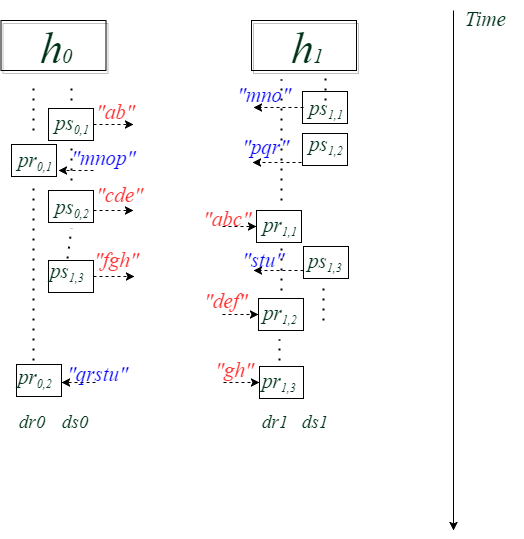
\includegraphics[scale=0.55]{Figures/reliableexample}}
\caption{Example of Reliable Communication}
\label{reliableexample}
\end{figure}

In this example, the payloads of the packages are:

$pl(pks_{01})=``ab"$, $ pl(pks_{02})=``cde"$, $pl(pks_{03})=``fgh"$;

$pl(pkr_{11})=``abc"$, $pl(pkr_{12})=``def"$, $pl(pkr_{13})=``gh"$ .

and 

$pl(pks_{11})=``mno"$, $pl(pks_{12})=``pqr"$, $pl(pks_{13})=``stu"$;

$pl(pkr_{01})=``mnop"$, $pl(pkr_{02})=``qrstu"$. 

on the other direction. 

Their properties:

$pl(pks_{01}) \cdot pl(pks_{02}) \cdot pl(pks_{03}) = pl(pkr_{11}) \cdot pl(pkr_{12}) \cdot pl(pkr_{13}) = ``abcdefgh"$ 

and

$pl(pks_{11}) \cdot pl(pks_{12}) \cdot pl(pks_{13}) = pl(pkr_{01}) \cdot pl(pkr_{02}) = ``mnopqrstu"$. 

satisfy the content preservation. 

The relative time relationship of the packages are: 

$time(pks_{01}) < time(pks_{02}) < time(pkr_{11})< time(pks_{03}) < time(pkr_{12}) < time(pkr_{13}) $;

$time(pks_{11}) < time(pks_{12}) < time(pkr_{01})< time(pks_{13}) < time(pkr_{02})$. 

The fact that
 
$pl(pkr_{01}) = ``mnop"$ is the prefix of $pl(pks_{11}) \cdot  pl(pks_{12}) = ``mnopqr"$,

$pl(pkr_{01}) \cdot pl(pkr_{02})=``mnopqrstu"$ is the prefix of (in this case is identical to ) $pl(pks_{11}) \cdot pl(pks_{12}) \cdot pl(pks_{13}) = ``mnopqrstu" $,  

$pl(pkr_{11})=``abc"$ is the prefix of $pl(pks_{01} \cdot pl(pks_{02}) = "abcde"$,  

$pl(pkr_{11}) \cdot pl(pkr_{12})= ``abcdef"$ and  $pl(pkr_{11}) \cdot pl(pkr_{12}) \cdot pl(pkr_{13}) = ``abcdefgh"$ are  the prefix of  $pl(pks_{01}) \cdot pl(pks_{02}) \cdot pl(pks_{03})= ``abcdefgh"$

satisfy the timing preservation. 


Figure\ref{unreliableexample} is an example of the unreliable communication. 

\begin{figure}[H]
\centerline{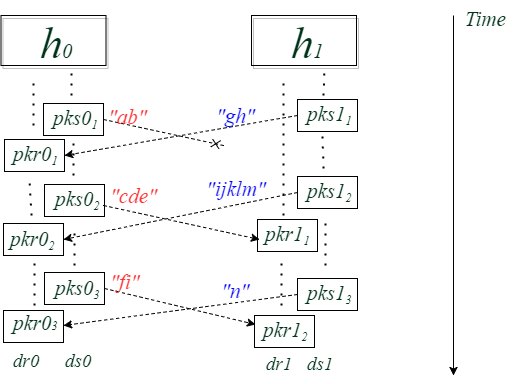
\includegraphics[scale=0.55]{Figures/unreliableexample}}
\caption{Example of Unreliable Communication}
\label{unreliableexample}
\end{figure}

In this example, the content preservation of the unreliable communication are satisfied since: 

$pkr_{11} = pks_{02}=``cde"$; 

$pkr_{12} = pks_{02}=``cde"$;

$pkr_{13} = pks_{03}=``fi"$;

$pkr_{01} = pks_{11}=``gh"$;

$pkr_{02} = pks_{12}=``ijklm"$;

$pkr_{03} = pks_{13}=``n"$.

while the timing preservation of the unreliable communication are satisfied since: 

$time(pkr_{11}) > time(pks_{02})$;

$time(pkr_{12}) > time(pks_{02})$; 

$time(pkr_{13}) > time(pks_{03})$;

$time(pkr_{01}) > time(pks_{11})$;

$time(pkr_{02}) > time(pks_{12})$;

$time(pkr_{03}) > time(pks_{13})$;




